\documentclass[10pt]{article}

% Nutze Times New Roman
\usepackage{newtxtext}
\usepackage{newtxmath}

\usepackage{graphicx}
\usepackage{url,hyperref}
\usepackage{multicol}
\usepackage[caption=false]{subfig}

\usepackage{geometry}
\geometry{a4paper, top=2cm, left=3cm, right=2cm, bottom=3cm}

\providecommand{\keywords}[1]
{
  \small	
  \textbf{\textit{Keywords---}} #1
}

\begin{document}

\title{Improved mirror ball projection for more accurate merging of multiple camera outputs}

\author{Yoko Hirono, Wladislav Artsimovich \\
	\\
	\href{mailto:wladislav.artsimovich@dmgmori.co.jp}{wladislav.artsimovich@dmgmori.co.jp}  \\
}

\maketitle

\begin{abstract}
	Using spherical mirrors in place of wide-angle cameras allows for close-up monitoring of manufacturing processes in hazardous environments, where a camera would normally not operate. This includes environments of high heat, vacuum and strong electromagnetic fields. Moreover, it allows the layering of multiple camera types (e.g., color image, near-infrared, long-wavelength infrared, ultraviolet) into a single wide-angle output, whilst accounting for the different camera placements and lenses used. Normally, the different camera positions introduce a parallax shift between the images, but with a spherical projection as produced by a spherical mirror, this parallax shift is strongly reduced and disappears almost completely with a mirror of a small size or if the monitoring target is some distance away from the mirror.

	This paper introduces a variation of the 'mirror ball projection', that accounts for distortion produced by a perspective camera at the pole of the projection. This distortion can make the alignment of multiple camera outputs inaccurate, especially if the camera distance to the spherical mirror is small. The new projection removes this error source.
\end{abstract}

\keywords{curved mirror, image registration, mirror ball, image processing, process monitoring, spherical projection}

\begin{figure}[h]
	\centering
	\subfloat[Caption]{
		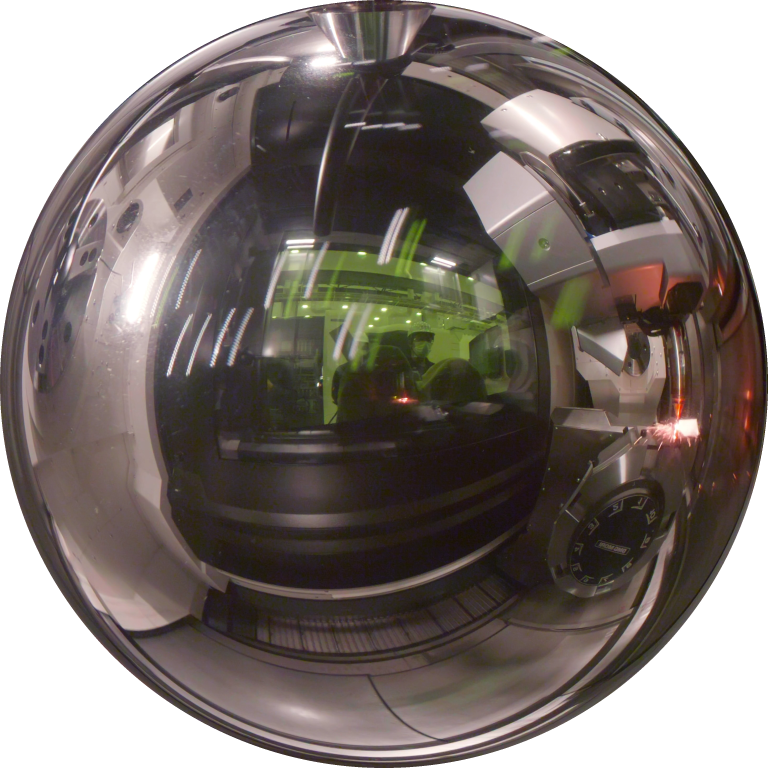
\includegraphics[width=0.23\textwidth]{img/multi_color.png}
		\label{fig:subfig1}
	}
	\hfill
	\subfloat[Caption]{
		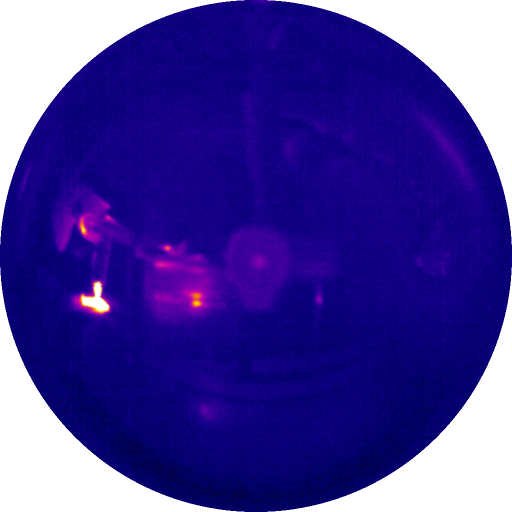
\includegraphics[width=0.23\textwidth]{img/multi_thermal.png}
		\label{fig:subfig2}
	}
	\hfill
	\subfloat[Caption]{
		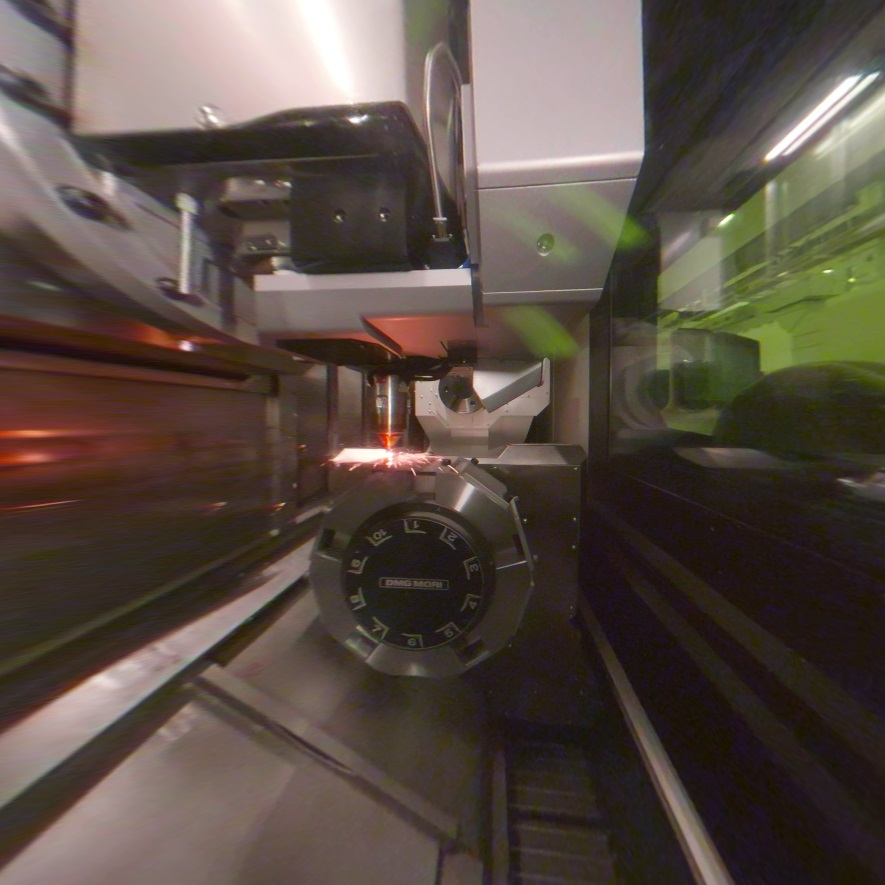
\includegraphics[width=0.23\textwidth]{img/projected_color.jpg}
		\label{fig:subfig3}
	}
	\hfill
	\subfloat[Caption]{
		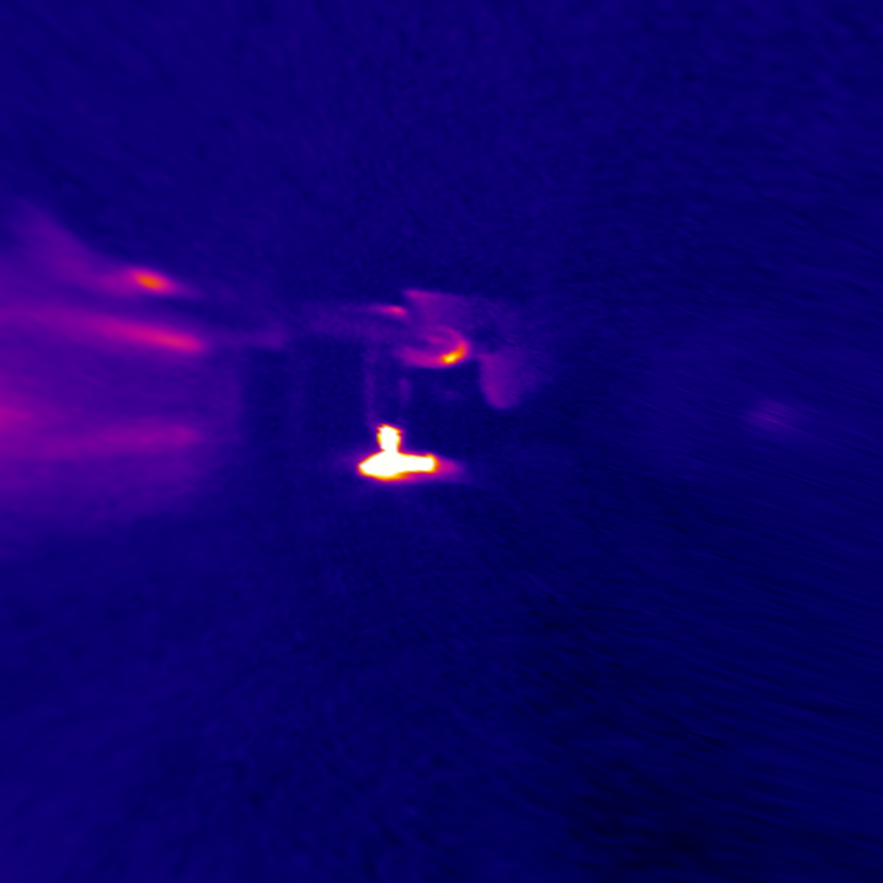
\includegraphics[width=0.23\textwidth]{img/projected_thermal.jpg}
		\label{fig:subfig4}
	}
\end{figure}

\begin{multicols}{2}
\section{Introduction}
Spherical mirror projections are used in a wide variety of applications as a substitute for wide-angle or panoramic camera systems. This extends to the field of robotics with omnidirectional camera systems \cite{omnidirectional} and to the field of computer graphics with various 'image-based lighting' techniques 2) or novel ways of displaying content 3). A less explored use case is process monitoring.

A mirror sphere is mathematically the simplest form of a spherical mirror and projects the full 360° environment onto a 2D plane, when captured with an orthographic camera. Whilst an orthographic camera can be achieved in the real-world with the use of a telecentric lens, almost all cameras are perspective ones. A distortion around the pole-point of the projection is introduced by merely approximating an orthographic camera when using a perspective one, especially at lower focal lengths.

What may make this projection an attractive option for process monitoring, is that the mirror itself can be made to withstand extreme conditions at relatively low cost. For instance, stainless steel ball bearings are a mass-produced commodity, that can survive high heat environments, whilst producing a mirror ball projection. Moreover, multiple cameras can be pointed at the same mirror sphere, all identically encoding the full 360° environment, regardless of camera position, at least mathematically. This allows for merging of multiple camera outputs into a single video feed, a technique referred to as 'image registration'.

\section{The projection term}
The mirror ball projection term, as used in this paper, maps a 3D reflection vector $\vec{r}$, as defined by the column vector, to the corresponding pixel on the 2D plane of an image, as defined by the column vector $\begin{bmatrix} {image}_x & {image}_y \end{bmatrix}^\intercal$. The origin of the coordinate system is at the center of the mirror ball, which itself is defined as a unit sphere, projecting onto the image plane as a unit circle. 

The term is a projection, which expresses a virtual camera-view at the center of an infinitely large sphere, allowing one to look around the full 360° environment, as reflected by the mirror surface of the imaged sphere.

\subsection{Deriving the classical mirror ball projection term}
The orthographic camera has its parallel view-rays defined by the incident ray column vector as written in Equation (1). As an orthographic camera captures the image, both the image's x,y-plane and the camera's x,y-plane are identical.
$$\vec{i}=\begin{bmatrix}
	0 & 0 & 1
\end{bmatrix}^\intercal$$
The law of reflection for a light ray hitting a smooth surface is defined by Eq. (2), with $\vec{r}$ being the reflected ray, $\vec{n}$ the surface normal and the dot '$\cdot$' being the scalar product.
$$ \vec{r}=2\left(\vec{i}\cdot\vec{n}\right)\vec{n}-\vec{i} $$
As per definition, the surface normal at each point of a unit sphere with its center at the origin, equals the vector as drawn from the origin to the surface at each point. With the orthographic camera's definition Eq. (1), the normal vector and the incident ray share the same xy-plane, leaving just the depth component of the normal $n_z$ as an unknown. Using that information, we can populate the law of reflection Eq. (2) and express the reflection vector $\vec{r}$ with the image's xy-plane:
$$\left[\begin{matrix}r_x\\r_y\\r_z\\\end{matrix}\right]=2\left(\left[\begin{matrix}0\\0\\1\\\end{matrix}\right]\cdot\left[\begin{matrix}{image}_x\\{image}_y\\n_z\\\end{matrix}\right]\right)\left[\begin{matrix}{image}_x\\{image}_y\\n_z\\\end{matrix}\right]-\left[\begin{matrix}0\\0\\1\\\end{matrix}\right]$$
Simplifying Eq. (3), it expresses this system of equations:
$$\left\{\begin{matrix}r_x=2n_z\ {image}_x\\r_y=2n_{z\ }{image}_y\\r_z=2{n_z}^2-1\ \ \ \ \ \\\end{matrix}\right.$$
However, we need this system the other way around. We want to get the correct image pixel, based on the reflection direction $\vec{r}$. Solving the 3rd equation of Eq. (4) for $n_z$, gives us
$$n_z=\ \sqrt{\frac{\left(r_z+1\right)}{2}}$$
Finally, we may substitute $n_z$ as defined by Eq. (5) into equation 1 and 2 of system Eq. (4). Simplifying the substitution gives us our mirror ball projection term:
$$\begin{bmatrix} image_x \\ image_y \end{bmatrix}=\frac{1}{\sqrt{2(r_z+1)}}\begin{bmatrix} r_x \\ r_y \end{bmatrix}$$

\subsection{Extending the projection term}
The classical projection term Eq. (6) suffers from distortion around the pole-point, as seen in Fig. 2b, because it assumes an orthographic camera. A perspective camera obscures part of the mirror sphere as a function of sphere radius and distance from the center. The true pole-point of the projection is thus not actually captured. 

The missing information can be conceived as the cone-shaped 'solid angle', defined by $2\pi-\alpha$, $\pi<\alpha<2\pi$, where $\alpha$ expresses the field of view in radians, that the mirror sphere is reflecting from the perspective of the camera's image. Any mapping from $\vec{r}$ going outside of the sphere's view cone will remain undefined. We need to remap the existing information to only fall within this cone. This can be achieved by stretching the reflection ray's image mapping by some scalar, specifically $\sin{\left(\frac{\alpha}{4}\right)}$. This ratio stems from the amount of surface representing the reflected information decreasing by the sine of the reflected angle divided by 4, as we go from the middle point of the sphere to its edges. By stretching the reflection rays and allowing them to become undefined when going past the image plane's unit circle, we rigidly define the missing information. This shows up as a black circle in place of the classical mirror ball projection's pole-point, depicted in Fig. 2c. Including said stretching scalar, results in the new and improved mirror ball projection term, shown in Equation (7). This term has been implemented in a demo WebApp, which can be accessed alongside sample photos and video footage on GitHub: \href{https://github.com/FrostKiwi/MirrorBall}{github.com/FrostKiwi/MirrorBall}
$$\begin{bmatrix} image_x \\ image_y \end{bmatrix}=\frac{1}{\sqrt{2(r_z+1)}\sin{\left(\frac{\alpha}{4}\right)}}\begin{bmatrix} r_x \\ r_y \end{bmatrix}$$

 \section{Process monitoring use case}
 Multiple camera views capturing the same mirror ball projection can be rotated into each other by a 3x3 rotation matrix, achieving image registration. Fig. 1a shows a mirror ball inside a DMG MORI 'LASERTEC 3000 DED hybrid' industry machine being captured using normal camera from the outside and a thermal camera from the inside of the machine. Fig 1b and 1c show the resulting mirror ball video feeds during laser cladding. Note, how both feeds show the hot metal sparks in different parts of the reflection. After correcting for the different rotations, both feeds are merged and can be switched between, as shown in figures Fig 1d and 1e. Even though the camera positions are different, the projections are at least mathematically in the exact same spot, thus having no parallax. Since these are 360° video feeds, they can be viewed with a VR headset, as shown in Fig. 2d. The captured $3k^2$ pixel resolution color image provides enough clarity to monitor the process, whilst the ability to switch to thermal vision in VR augments the monitoring experience.

\section{Conclusion}
This paper extended the classical mirror sphere projection term by a new distortion scalar $\sin{\left(\frac{\alpha}{4}\right)}$ and its field of view parameter $\alpha$. This parameter allows one to express the distortion numerically, that is introduced by a perspective camera, when capturing a mirror ball projection. By counteracting this distortion, a more accurate registration of multiple camera outputs was achieved, when capturing the same mirror ball projection from different viewpoints.

\bibliographystyle{abbrv}
\bibliography{references}
\end{multicols}
\end{document}
